\documentclass[12pt,aspectratio=169]{beamer}
% \hypersetup{pdfpagemode=FullScreen}

\renewcommand*{\thefootnote}{\fnsymbol{footnote}}

\mode<presentation>
\useoutertheme[subsection=false]{miniframes}

\title{GDP: Generalized Device Placement For Dataflow Graphs}
\author{Yanqi Zhou \and %
        Sudip Roy \and %
        Admirali Abdolrashidi \and %
        Daniel Wong \and \\ %
        Peter C. Ma \and %
        Qiumin Xu \and %
        Ming Zhong \and %
        Hanxiao Liu \and \\ %
        Anna Goldie \and %
        Azalia Mirhoseini \and %
        James Laudon}%
\institute{Google Brain}
\date{Jan 9, 2020}

\begin{document}
    \beamertemplatenavigationsymbolsempty
    
    \begin{frame}
        \titlepage
    \end{frame}

    \section{Introduction}

    \begin{frame}
        \frametitle{Introduction}

        Neural networks have demonstrated remarkable scalability – improved performance can usually be achieved by
        training a larger model on a larger dataset. Training such large models efficiently while meeting device
        constraints, like memory limitations, necessitate partitioning of the underlying dataflow graphs for the models
        across multiple devices.
    \end{frame}

    \begin{frame}
        \frametitle{Device Placement Using Reinforcement Learning}

        \begin{itemize}
            \setlength{\itemsep}{1.4em}
            \item \textbf{HDP} (Mirhoseini et al., 2018) uses feed forward NN to assign each op to a group and runs a
                  seq-to-seq model to place each group to a device.
            \item \textbf{Spotlight} (Gao et al., 2018) heuristically groups nodes and generates placements with LSTM.
            \item \textbf{Placeto} (Addanki et al., 2019) uses GNN to encode the graph structure into embeddings, then
                  uses feed forward NN to iteratively generate a placement for one node at each step.
            % HDP uses feature of nodes in the first layer, but Spotlight ignores them and only use op name as input.
        \end{itemize}
    \end{frame}

    \begin{frame}
        \frametitle{GDP}

        \begin{itemize}
            \setlength{\itemsep}{.8em}
            \item An end-to-end deep RL method for device placement that can generalize to arbitrary and held-out graphs.
            \item The placement network is 15x faster than HDP without the need for explicit grouping.
            \item A new batch pre-training and fine-tuning strategy based on network superposition, which leads to
                  improved transferability, better placements especially for large graphs, and huge reduction in policy
                  search time.
            \item Superior performance over a wide set of workloads including graphs with over 50k nodes.
        \end{itemize}
    \end{frame}

    \section{System Design}

    \begin{frame}
        \frametitle{Problem Formulation}

        Given a dataflow graph $G(V, E)$ where $V$ represents atomic computational operations (ops) and $E$ represents
        the data dependency. The goal of GDP is to learn a policy $\pi: \mathcal{G} \mapsto \mathcal{D}$ that maximizes
        reward $r_{G,D}$ defined based on the run time. GDP represents policy $\pi_\theta$ as a nerual network
        parameterized by $\theta$.

        $$
            J(\theta) = \mathbb{E}_{G\sim{} \mathcal{G}, D\sim \pi_\theta(G)}[r_{G,D}] \approx
            \frac{1}{N}\sum_{G}\mathbb{E}_{D\sim \pi_\theta(G)}[r_{G,D}]
        $$

        We refer to the case when $N=1$ as \textit{individual training} and the case when $N>1$ as \textit{batch training}.
    \end{frame}

    \begin{frame}
        \frametitle{System Overview}

        \centering
        \includegraphics[page=3,trim=4.5cm 21cm 4.5cm 3cm,clip]{GDP.pdf}

        \vskip .1em
        $N$: Number of nodes, $h$: Hidden Size, $d$: Number of Devices
    \end{frame}

    \begin{frame}
        \frametitle{Graph Embedding Network}

        GDP adopts the feature aggregation scheme proposed in \textit{GraphSAGE} as it shows better generalization.
        \begin{align*}
            h^{(l)}_{\mathcal{N}(v)} &= \text{max}(f_a^{(l)}(h^{(l)}_u), \forall u \in \mathcal{N}(v)) \\
            h^{(l+1)}_v &= f_b^{(l+1)}(\text{concat}(h^{(l)}_v, h^{(l)}_{\mathcal{N}(v)}))
        \end{align*}

        where $h_v$ is the hidden feature of $v$, $f_a$ and $f_b$ are dense layers, $\mathcal{N}(v)$ represents the
        neighbors of $v$, and $h_{\mathcal{N}(v)}$ stands for the aggregated feature from the neighbors of $v$.

        \vskip 1em
        Different from GraphSAGE, which is unsuperised, GDP trains the embeddings jointly with the placement network.
    \end{frame}

    \begin{frame}
        \frametitle{GraphSAGE}

        \centering
        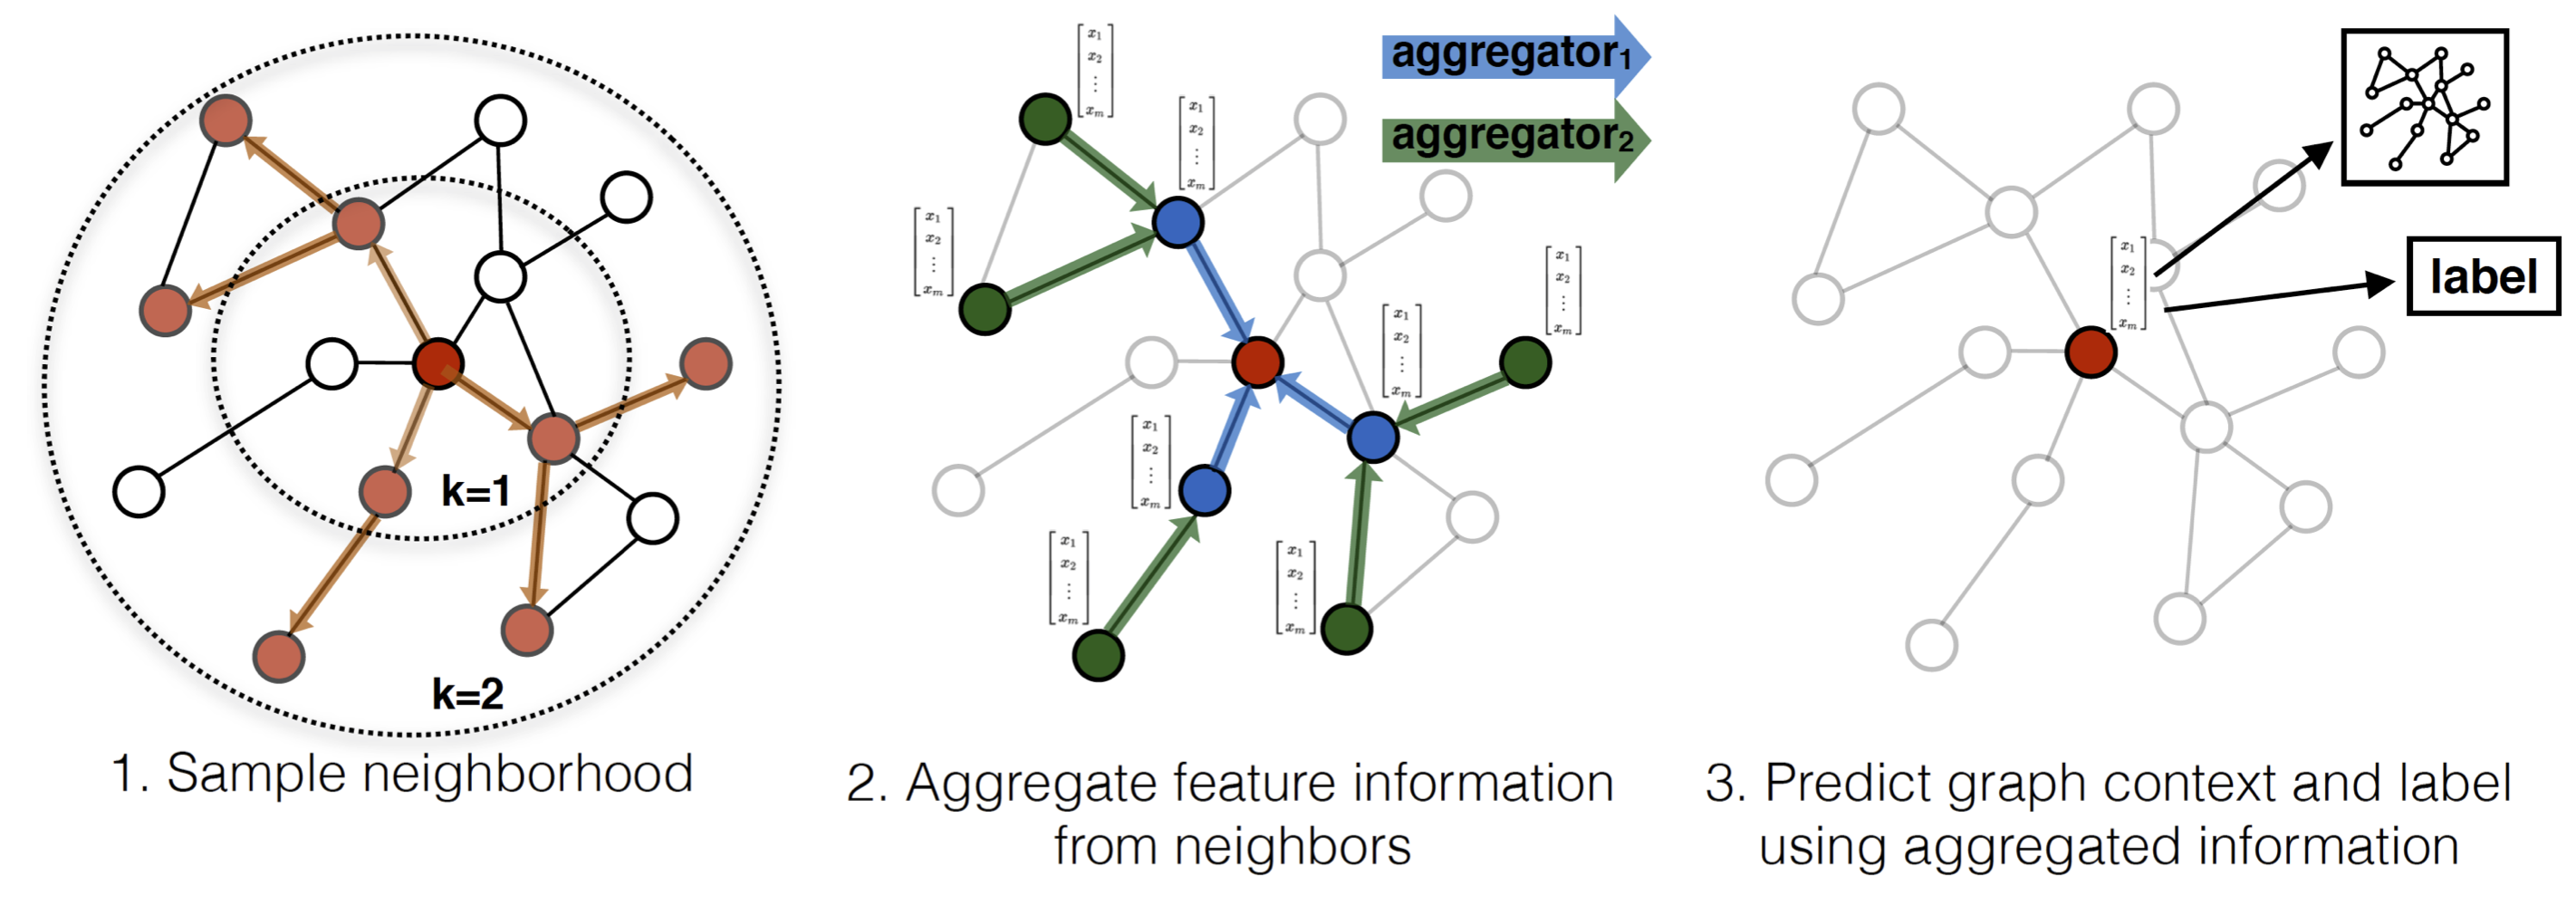
\includegraphics[width=\textwidth]{graphsage.png}
    \end{frame}

    \begin{frame}
        \frametitle{Placement Network}

        \begin{itemize}
            \setlength{\itemsep}{.8em}
            \item Conventional seq-to-seq models usually target short sequences, which requires grouping beforehand.
            \item LSTM used in previous works is slower and more difficult to train than attention-based models.
            \item GDP adopts segment-level recurrence introduced in \textit{Transformer-XL} to capture long-term
                  dependencies. The key is to cache (with gradient flows disabled) and reuse the hidden states of
                  previous segments.
        \end{itemize}
    \end{frame}

    \begin{frame}
        \frametitle{Transformer XL}

        \centering
        \includegraphics[page=3,trim=2.6cm 23.8cm 2.6cm 2.2cm,clip,scale=.88]{transformerxl.pdf}
        \vskip .2em
        \includegraphics[page=4,trim=2.5cm 23.8cm 2.7cm 2.2cm,clip,scale=.88]{transformerxl.pdf}
    \end{frame}

    \begin{frame}
        \frametitle{Batch Training}

        \begin{itemize}
            \item Naive batch training is challenging because of the divergence of the dataflow graphs.
            \item GDP uses a feature conditioning mechanism similar to \textit{parameter superposition}, implemented by
                  replacing all dense layers in the placement network with:
        \end{itemize}
        
        $$ x^{(l+1)} = g^{(l)}(c(x^{(0)}) \odot x^{(l)}) $$

        \vskip 1em
        \hspace{1.9em} where $g^{(l)}$ stands for a dense layer in the placement network, $c$ stands for the feature
        conditioning layer, and $x^{(0)}$ denotes the input feature generated by the graph-embedding network.

        % In the paper of superposition, c is c^l, which means x^l may have different length.
    \end{frame}

    \section{Experiment}

    \begin{frame}
        \frametitle{Experiment Setup}

        \begin{itemize}
            \setlength{\itemsep}{1.4em}
            \item We compare GDP with human expert placement (\textbf{HP}), Tensorflow \textbf{METIS} placement (a
                  general purpose graph partitioning tool), and \textbf{HDP} (Mirhoseini et al., 2018).
            \item 8 Nvidia P100
            \item We use negative square root of the run time as the reward, and subtract the average reward of all
                  previous trials to calculate the advantage value. Invalid placements are given a large (-10) negative
                  reward.
        \end{itemize}
    \end{frame}

    \begin{frame}
        \frametitle{Performance on Individual Graphs}

        \centering
        \includegraphics[page=6,trim=3cm 15cm 3cm 5cm,clip,scale=.88]{GDP.pdf}
    \end{frame}

    \begin{frame}
        \frametitle{Performance on Batch Training}

        \begin{center}
        Run time comparing on GDP-batch vs. GDP-one
        \vskip .2em
        \includegraphics[page=7,trim=5cm 21.2cm 5cm 3.6cm,clip]{GDP.pdf}
        \end{center}

        A possible explanation for the performance gain is the additional feature conditioning layer in the batch
        training effectively enlarged the model.
        % Batch training adds a conditioning layer for very dense layer, effectively enlarged the network by 2x.
    \end{frame}

    \begin{frame}
        \frametitle{Performance on Hold-out Graphs}

        We run GDP on unseen graphs with and without finetuning, called \textbf{GDP-gereralization-finetune} and
        \textbf{GDP-gereralization-zeroshot} respectively.

        \vskip 1em
        \centering
        \includegraphics[page=7,trim=5cm 12.9cm 5cm 9.6cm,clip]{GDP.pdf}
    \end{frame}

    \begin{frame}
        \frametitle{Ablation Studies}

        We did ablation studies on the attention and the superposition layer in the placement network. They improved the
        average run time by 18\% and 6.5\% respectively.

        \vskip 1em
        \centering
        \includegraphics[page=8,trim=4cm 20cm 4cm 3.2cm,clip]{GDP.pdf}
    \end{frame}

    \begin{frame}
        \frametitle{Pre-training Graph Embeddings}

        We train GDP-batch like before, but then fine-tuning on each specific graphs. The run time and search time
        are reduced by 5\% and 86\% respectively, compared with GDP-one.

        \centering
        \includegraphics[page=8,trim=6.4cm 12.5cm 5.8cm 9.8cm,clip]{GDP.pdf}
    \end{frame}

    \appendix

    \begin{frame}
        \vskip 1.5em

        \centering \huge
        Thank you!
    \end{frame}
\end{document}